\documentclass[11pt,a4paper]{article}
\usepackage[margin=2.2cm]{geometry}
\usepackage{fontspec}
\setmainfont{TeX Gyre Pagella}
\setmonofont{DejaVu Sans Mono}[Scale=0.82]
\usepackage{amsmath,amssymb,amsthm}
\usepackage{graphicx,xcolor,listings,booktabs,enumitem}
\usepackage[most]{tcolorbox}
\usepackage{tikz}
\usepackage[hidelinks]{hyperref}

\definecolor{accent}{HTML}{2B6CB0}
\definecolor{warn}{HTML}{C53030}
\newtcolorbox{keybox}[1][]{colback=accent!5,colframe=accent,boxrule=0.6pt,arc=2pt,left=6pt,right=6pt,top=4pt,bottom=4pt,#1}
\newtcolorbox{warnbox}{colback=warn!5,colframe=warn,boxrule=0.6pt,arc=2pt,left=6pt,right=6pt}

\lstdefinelanguage{Rust}{
  keywords={fn,let,mut,if,else,for,in,while,return,use,pub,struct,impl,loop,break,Some,None,as,match,const,Self,self},
  morekeywords=[2]{usize,i32,i64,u64,f64,bool,Vec,VecDeque,BTreeSet,BTreeMap,BinaryHeap,Option,str},
  sensitive=true, morecomment=[l]{//}, morestring=[b]"}
\lstset{language=Rust,basicstyle=\ttfamily,keywordstyle=\color{accent}\bfseries,
  keywordstyle=[2]\color{teal},commentstyle=\color{gray}\itshape,stringstyle=\color{warn},
  frame=single,rulecolor=\color{gray!40},backgroundcolor=\color{gray!4},
  numbers=left,numberstyle=\tiny\color{gray},xleftmargin=1.5em,breaklines=true,
  columns=fullflexible,keepspaces=true,showstringspaces=false}

\newtheorem*{invariant}{Invariant}
\theoremstyle{definition}\newtheorem*{definition}{Definition}

\usepackage{soul}
\definecolor{hlY}{HTML}{FFF3A0}\definecolor{hlG}{HTML}{C8F2C2}\definecolor{hlP}{HTML}{E6D2F7}\definecolor{hlB}{HTML}{CFE3FF}
\newcommand{\hly}[1]{{\sethlcolor{hlY}\hl{#1}}}
\newcommand{\hlg}[1]{{\sethlcolor{hlG}\hl{#1}}}
\newcommand{\hlp}[1]{{\sethlcolor{hlP}\hl{#1}}}
\newcommand{\hlb}[1]{{\sethlcolor{hlB}\hl{#1}}}
\newcommand{\img}[3]{\begin{center}\fcolorbox{gray!50}{white}{\includegraphics[width=#1]{board/#2}}\\[-2pt]{\footnotesize\textcolor{gray}{#3}}\end{center}}
\newcommand{\board}[3]{\img{#1}{#2}{Board, #3 (recording \texttt{L\_10.MP4})}}
\newcommand{\extra}{\textsuperscript{\textcolor{warn}{[extra]}}}
% pages of the prof's 2025 notes on prefix sums (Lessons/L10/Prefix_sums_2025.pdf)
\newcommand{\oldnotes}[3]{\begin{center}\fcolorbox{gray!50}{white}{\includegraphics[page=#1,width=#2,trim=0 #3 190 0,clip]{Prefix_sums_2025.pdf}}\\[-2pt]
  {\footnotesize\textcolor{gray}{Prof.'s notes of \textbf{last year} (2025), \texttt{Prefix\_sums\_2025.pdf} p.\,#1}}\end{center}}
\title{\textbf{CPC --- Lecture 10}\\[2pt]\large Little Girl and Maximum Sum $\cdot$ Number of Ways $\cdot$ Fenwick tree (start)}
\author{Competitive Programming and Contests --- Monday 19/10/2026}
\date{}

\begin{document}\sloppy
\maketitle
\vspace{-1.5em}
\begin{keybox}
\textbf{Sources.} Recording \texttt{Lessons/L10/L\_10.MP4} (85 min) and its automatic transcript \texttt{L10\_transcript.txt} (not revised);
the prof's handwritten board (frames of the recording, \texttt{board/l10\_*.jpg});
the prof's 2025 notes \texttt{Lessons/L10/Prefix\_sums\_2025.pdf} (static prefix sums, Ilya, Little Girl, Number of Ways);
the prof's blog posts \emph{The Power of Prefix Sums} (\url{https://pages.di.unipi.it/rossano/blog/2023/prefixsums}) and
\emph{Dynamic Prefix Sums with Fenwick Tree} (\url{https://pages.di.unipi.it/rossano/blog/2023/fenwick}), code copied verbatim;
your notes \texttt{Lessons/L10/notes.md}.
\hlp{The recording stops at 84:54, in the middle of the Fenwick tree} (the iPad was running out of battery): the last part of \S\ref{sec:fenwick}
comes \textbf{only from your notes} and is marked as such.
Everything marked \extra{} was \emph{not} said or written in the lecture (my explanations, examples, code).

\smallskip
\noindent Code: \texttt{Lessons/L10/src} (\texttt{cargo test -p l10}). Exercises: \texttt{Lessons/L10/practice}, E43--E46 (\texttt{cargo test -p practice\_l10}).

\smallskip
\noindent\textbf{Highlights:} \hly{general / to remember} \quad \hlg{good: works, efficient, correct} \quad \hlp{bad: pitfalls, wrong ideas, costs} \quad \hlb{definitions and key results}
\end{keybox}

\begin{keybox}[colback=gray!4,colframe=gray!60]
\textbf{Where we are.} L9 (14/10) ended Frogs and Mosquitoes and solved the first static prefix-sum problem, \emph{Ilya and Queries} (``problem \#1'').
Today: \textbf{problem \#2} \emph{Little Girl and Queries} and \textbf{problem \#3} \emph{Number of Ways}, ``the last problem about static prefix sums'',
then the start of \textbf{dynamic prefix sums} with the \textbf{Fenwick tree}. (This explains the numbering in your notes: the ``problem \#2'' you could not find is Little Girl.)
\end{keybox}

\tableofcontents

%==========================================================
\section{Problem \#2: Little Girl and Queries (Codeforces 276C)}
%==========================================================
\subsection{The problem}
\textbf{Problem.} Given an array $A[1,n]$ and a set $Q$ of $m$ queries, each query a $\textsf{RangeSum}(i,j)$.
\hlb{Permute the values of \mbox{$A$} to maximize the sum of the results of the queries in \mbox{$Q$}}
(``we are free to permute the elements in any way we want; the elements must remain the same'').

\noindent\textbf{Example.} $A=[5,2,4,1,3]$, queries $(1,5)$, $(2,3)$, $(2,3)$: value $15+6+6=27$
(the prof says ``26'' at 03:56, a slip: the board says 27). With $A^\pi=[2,5,4,1,3]$: $15+9+9=\mathbf{33}$, which is the optimum.
\board{0.62\textwidth}{l10_little_example.jpg}{10:00}
\noindent\hlb{Target time complexity: \mbox{$\Theta(n\log n+m\log m)$}} (board; ``can be improved a bit, we will discuss later'').
\extra{} Your notes write the two short queries as $(1,2)$: on the board they are under the values $2,4$, i.e.\ positions $2,3$.

\subsection{The idea (found in class)}
\hlb{For every position count how many queries touch it (its \emph{frequency}); put the largest values in the most frequent positions.}
In the example the frequencies are $1,3,3,1,1$: $5$ and $4$ go to positions $2,3$, then $1,2,3$ anywhere $\Rightarrow 15+9+9=33$.
\begin{itemize}[nosep]
\item \textbf{Step \#1}: count the frequency of every position.
\item \textbf{Step \#2}: sort $A$ in decreasing order, $\Theta(n\log n)$; sort the pairs (frequency, position) in decreasing order, $\Theta(m\log m)$ on the board
      \extra{} (there are $n$ pairs, so strictly $\Theta(n\log n)$); assign the greatest value to the most frequent position.
\end{itemize}
\board{0.62\textwidth}{l10_little_steps.jpg}{16:00}
\noindent\hly{Remark: with constraints on the values of \mbox{$A$}, or on \mbox{$m$} (frequencies are \mbox{$\le m$}), counting sort removes the logarithmic factors.}

\subsection{Step \#1, solution 1: sweep line --- $\Theta(n+m\log m)$}
Proposed by a student, ``something we already discovered'' in the \emph{maximum number of overlapping intervals} problem (L7):
\hly{sort the begin/end points of the segments, move the sweep line, \mbox{$+1$} at every beginning, \mbox{$-1$} at every end}; here we can also scan
all the $n$ positions to write down every frequency. Cost: \hlp{\mbox{$\Theta(m\log m)$} for sorting} the $2m$ endpoints. (The prof did not write this one on the iPad.)

\subsection{Step \#1, solution 2: an array whose prefix sums are $F$ --- $\Theta(n+m)$}
``Very useful because we are going to reuse the idea later.'' Queries $(2,4)$, $(1,3)$, $(2,5)$ on $n=5$: the target is $F=[1,3,3,2,1]$.
\hlb{Build an array \mbox{$B$} such that its prefix sums are \mbox{$F$}.}
\begin{itemize}[nosep]
\item A $+1$ in $B[i]$ is propagated by the prefix sums \emph{until the end} of the array: $+1$ at 2 gives $0,1,1,1,1$.
\item The segment $(2,4)$ should give $0,1,1,1,0$: we must stop the propagation \hly{at the position immediately after the end of the segment, with a \mbox{$-1$}}.
\item So every query $(i,j)$ does \hlb{\mbox{$B[i]\mathrel{+}=1$} and \mbox{$B[j+1]\mathrel{-}=1$}} (nothing if $j+1>n$). Then $F$ = prefix sums of $B$.
\end{itemize}
Example: $B=[1,2,0,-1,-1]\Rightarrow F=[1,3,3,2,1]$. (The prof made a mistake on the first try, putting a $-1$ at the end instead of after it,
and redid it from scratch: \hlp{the \mbox{$-1$} goes at \mbox{$j+1$}, not at \mbox{$j$}}.)
\hlg{Time \mbox{$\Theta(n+m)$}}: zero out $B$, two updates per query, one prefix-sum pass. \hlg{Better than the sweep line}, which sorts.
\board{0.55\textwidth}{l10_little_B.jpg}{36:20}

\noindent\textbf{But the sweep line can be linear too: counting sort.} Do we really need a comparison-based sort ($m\log m$) for the endpoints? No:
\hly{the largest possible endpoint is \mbox{$n$}, so counting sort with an array of \mbox{$n$} counters works}. We must keep the
\emph{satellite information} (beginning or end?): either $2n$ counters, or two arrays $C_b$ (beginnings) and $C_e$ (ends).
In the example $C_b=[1,2,0,0,0]$, $C_e=[0,0,1,1,1]$ (positions of the ends).
\hlb{\mbox{$B$} is just a more direct representation of \mbox{$C_b$} and \mbox{$C_e$}}: $+1/-1$ instead of ``beginning/end''. And the (stable) counting sort
is itself doing prefix sums, to find where the elements equal to a key end in the sorted array: ``we are rediscovering the same approaches often''.
\oldnotes{5}{0.5\textwidth}{470}

\begin{keybox}
\textbf{Lesson (``I would like to remark this'').} \hlb{Always consider the magnitude of the values in your task.} If the numbers are bounded,
direct-access tables instead of hashing, counting sort / radix sort instead of merge sort: much faster.
\end{keybox}

\noindent\textbf{Prof's code} [blog] (verbatim; \texttt{l10::little\_girl}):
\begin{lstlisting}
// We assumes queries are 0-based indexed
pub fn little_girl(a: &[i64], q: &[(usize, usize)]) -> i64 {
    if a.is_empty() {
        return 0;
    }

    let mut u = vec![0i64; a.len()];

    for &(l, r) in q {
        assert!(l <= r);
        assert!(r < u.len());

        u[l] += 1;
        if r + 1 < u.len() {
            u[r + 1] -= 1;
        }
    }

    let mut f = u
        .iter()
        .scan(0, |sum, e| {
            *sum += e;
            Some(*sum)
        })
        .collect::<Vec<_>>();

    // we sort both f and a in decreasing order, nothing changes
    f.sort_unstable();
    let mut a_sorted = a.to_vec();
    a_sorted.sort_unstable();

    a_sorted
        .iter()
        .zip(f)
        .fold(0, |result, (value, freq)| result + value * freq)
}
\end{lstlisting}
\noindent\extra{} \texttt{u} is the array $B$. Both arrays are sorted in \emph{increasing} order: pairing the $k$-th smallest with the $k$-th smallest is the same as pairing
the largest with the largest. Total: $\Theta(m+n\log n)$.

%==========================================================
\section{Problem \#3: Number of Ways (Codeforces 466C)}
%==========================================================
``The last problem about \emph{static} prefix sums'' (static: the array does not change after computing the prefix sums).

\noindent\textbf{Problem.} Given $A[1,n]$, count \hlb{in how many ways we can split \mbox{$A$} into 3 parts so that the sums of the parts are the same}.
\hly{To make it interesting, the values can be zero or negative}: \hlp{with positive values only there is at most one split} (just check 0 or 1).

\noindent\textbf{Example.} $A=[1,2,3,0,3]$: 2 ways, $[1,2\,|\,3\,|\,0,3]$ and $[1,2\,|\,3,0\,|\,3]$, all parts sum to 3.
\board{0.42\textwidth}{l10_ways_example.jpg}{42:00}
\noindent Target: \hlb{linear time}.

\subsection{Cubic and quadratic}
Cubic: try all the splittings and compute the sums. Quadratic: $S$ = sum of $A$, \hly{target \mbox{$T=S/3$}}; with prefix sums,
\hly{fix the central part \mbox{$[i,j]$}} (quadratically many) and check $\textsf{RangeSum}(i,j)=T$ in $O(1)$. If it is, the prefix and the suffix sum to $2T$ together:
check that the prefix is $T$ (then the suffix is $T$ too, the total being $3T$).

\subsection{Linear}
The class went towards two pointers, then towards counting. Summary given by the prof:
\begin{enumerate}[nosep]
\item Left to right, compute the prefix sums and \hly{mark with ``+'' (blue) every position where the prefix sum is \mbox{$T$}}: each one is the end of a valid first part.
      ``We may have many of them'' (zeros and negative numbers).
\item For each ``+'' we want \hly{how many splits of the remaining suffix into 2 parts of sum \mbox{$T$} each}, and sum these numbers. It is not enough to find one $j$,
      and \hlp{scanning the remaining part for every ``+'' is quadratic}.
\item Right to left, compute suffix sums and \hly{mark with a (red) dot every position where the suffix sum is \mbox{$T$}}: the beginning of a valid third part.
      Then the middle part sums to $3T-T-T=T$ automatically.
\item \hlb{Answer = \mbox{$\sum$} over the ``+'' of the number of red dots to its right.} \hlp{Not ``\#blue \mbox{$\times$} \#red''}: that counts pairs with the red dot on the left (double counting).
\item ``How many red points on the right?'' is \hlg{a suffix sum on 0/1 indicators} (1 if the position is red): precomputed, \hlg{\mbox{$\Theta(n)$} overall}.
\end{enumerate}
\board{0.55\textwidth}{l10_ways_marks.jpg}{59:40}
\noindent\extra{} ``To the right'' must leave a non-empty middle part: if the first part ends at $i$, the third part starts at $\ge i+2$.
Last year the prof also warmed up with the easier problem of splitting into \emph{2} parts (one scan, check $p=S/2$): not done this year, see p.\,6 of the 2025 notes.

\noindent\textbf{Prof's code} [blog] (verbatim; \texttt{l10::number\_of\_ways}):
\begin{lstlisting}
pub fn number_of_ways(a: &[i64]) -> usize {
    let sum: i64 = a.iter().sum();

    if sum % 3 != 0 {
        return 0;
    }

    let target = sum / 3;
    let mut c: Vec<_> = a
        .iter()
        .rev()
        .scan(0, |sum, e| {
            *sum += e;
            Some(*sum)
        })
        .scan(0, |counter, sum| {
            if sum == target {
                *counter += 1usize
            };
            Some(*counter)
        })
        .collect();

    c.reverse();

    let mut result = 0;
    let mut sum = 0;
    for (i, &v) in a[..a.len() - 2].iter().enumerate() {
        sum += v;
        if sum == target {
            result += c[i + 2];
        }
    }

    result
}
\end{lstlisting}
\noindent\extra{} $c[i]$ = number of red dots at positions $\ge i$ (the suffix sum on the indicators); \texttt{c[i + 2]} leaves at least one element in the middle.
\hlp{Pitfall: with \mbox{$n=1$} (allowed by Codeforces) \texttt{a.len() - 2} underflows and the function panics} (\texttt{number\_of\_ways(\&[0])}); guard with
\texttt{if a.len() < 3 \{ return 0; \}}. Tested in \texttt{l10} against an $O(n^2)$ brute force.

%==========================================================
\section{Dynamic prefix sums: the Fenwick tree}\label{sec:fenwick}
%==========================================================
\subsection{Why it matters}
``One of the most elegant data structures we are going to see in this course.''
\begin{itemize}[nosep]
\item \hlb{Both operations in \mbox{$O(\log n)$}}, ``just three instructions per operation'', very fast.
\item \hlg{No more space than the array it indexes}: \hly{implicit} --- a binary tree stored in an array, the structure is in the order of the elements, and we move
      between parent and children with \hly{binary operations on the index} (hence the other name, \textbf{Binary Indexed Tree, BIT}).
\item Alternative: the \textbf{segment tree} (coming next): same time, \hlp{more space}, but \hlg{easy to modify for other operations} (minimum of a subarray, \dots).
      The Fenwick tree is mostly used for dynamic prefix sums.
\item Named after its inventor, P.\ Fenwick (New Zealand), who used it for \emph{arithmetic coding}: while scanning a text you keep the frequencies of the symbols
      updated and need how many occurrences of symbols smaller than $b$ there are, i.e.\ prefix sums on dynamic frequencies.
\end{itemize}

\subsection{The problem and the trivial solutions}
Given $A[1,n]$, support \hlb{\mbox{$\textsf{Sum}(i)=\sum_{k=1}^{i}A[k]$} and \mbox{$\textsf{Add}(i,v)$}: \mbox{$A[i]\mathrel{+}=v$}} ($v$ may be negative).
$\textsf{RangeSum}(i,j)=\textsf{Sum}(j)-\textsf{Sum}(i-1)$, so we only discuss \textsf{Sum} (``easier to implement'').
\begin{center}
\begin{tabular}{lcc}\toprule
 & \textsf{Sum}$(i)$ & \textsf{Add}$(i,v)$ \\\midrule
store $A$ & \hlp{$\Theta(n)$} & $O(1)$ \\
store the prefix sums of $A$ & $O(1)$ & \hlp{$\Theta(n)$} (all following prefix sums change) \\
\textbf{BIT} & \hlg{$\Theta(\log n)$} & \hlg{$\Theta(\log n)$} \\\bottomrule
\end{tabular}
\end{center}
\board{0.5\textwidth}{l10_fenwick_trivial.jpg}{72:40}
\noindent\hly{The trivial solutions are useful only with a huge imbalance}: one operation done a linear number of times and the other asymptotically fewer than
$\log n$ times (or, a student noted, a group of all the adds followed by all the sums). In any other case, the vast majority, the BIT is better.

\subsection{Relaxed version: Sum only at powers of two}
Running example (``for a while''): $A=[3,2,-1,5,7,-3,2,1]$, positions $1..8$.
\begin{itemize}[nosep]
\item \textbf{Relaxed problem}: $\textsf{Sum}(i)$ \hly{only if \mbox{$i$} is a power of 2} (undefined otherwise); $\textsf{Add}(i,v)$ for every $i$.
\item Checklist entry for data-structure problems: \hlb{how many possible questions are there? If few, precompute the answers.} Here only $\log n$ positions can be asked:
      store $\textsf{Sum}(1)=3$, $\textsf{Sum}(2)=5$, $\textsf{Sum}(4)=9$, $\textsf{Sum}(8)=16$.
\item $\textsf{Sum}$: \hlg{\mbox{$O(1)$}}. $\textsf{Add}(i,v)$: update the stored answers at the powers of two $\ge i$, \hlg{\mbox{$O(\log n)$}} (worst case $i=1$, all of them change).
      Example: $\textsf{Add}(6,5)$ changes only position 8: $16\to21$.
\item ``I promised a tree'': add a \hly{fake root (position 0, value 0)} and connect it to the stored nodes. Write the range of each node, $[1,1],[1,2],[1,4],[1,8]$,
      and the positions in binary: $0001,0010,0100,1000$. ``What's the characteristic of these positions?'' \extra{} \hlb{exactly one bit set to 1}.
\end{itemize}
\board{0.45\textwidth}{l10_fenwick_relaxed.jpg}{84:00}

\subsection{After the recording: from your notes}
\begin{warnbox}
\textbf{The recording ends here (84:54).} What follows is from your notes only (\texttt{notes.md}); figure and \extra{} parts are mine.
To be checked against L11 if the prof recaps.
\end{warnbox}
\begin{itemize}[nosep]
\item \hly{Cover the uncovered parts by applying the same principle recursively.} Between 4 and 8 the uncovered part is $[7,-3,2]$ (positions $5,6,7$, i.e.\ $1,2,3$ shifted by 4):
      its relaxed solution stores $[5,5]=7$ and $[5,6]=4$, positions $0101$ and $0110$ (\hlb{two bits set}), linked to their parent, node 4.
      Then $[-1]$ at position $3=0011$, range $[3,3]$, child of node 2; and \extra{} $2$ at position $7=0111$, range $[7,7]$, child of node 6.
\item \hlb{Number of trailing 0s in the binary representation of a node = number of its children.}
\item $\textsf{Sum}(i)$: start from the node whose range ends at $i$ (node $i$) and \hly{sum its value and the values of its ancestors up to the root}.
\item $\textsf{Add}(i,v)$: \hly{update the values of all the nodes whose range contains \mbox{$i$}}. (Running times: not written in your notes.)
\end{itemize}

\noindent\extra{} The whole tree of the example (value, range, position in binary):
\begin{center}
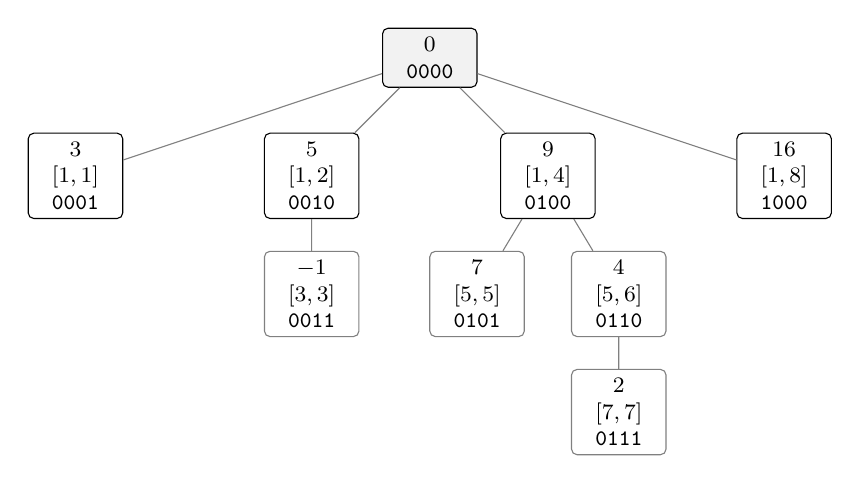
\begin{tikzpicture}[every node/.style={draw,rounded corners=2pt,align=center,font=\footnotesize,minimum width=12mm},
  level distance=15mm, level 1/.style={sibling distance=30mm}, level 2/.style={sibling distance=18mm}, level 3/.style={sibling distance=15mm}, edge from parent/.style={draw,gray}]
\node[fill=gray!10] {0\\\texttt{0000}}
  child {node {3\\$[1,1]$\\\texttt{0001}}}
  child {node {5\\$[1,2]$\\\texttt{0010}}
     child {node {$-1$\\$[3,3]$\\\texttt{0011}}}}
  child {node {9\\$[1,4]$\\\texttt{0100}}
     child {node {7\\$[5,5]$\\\texttt{0101}}}
     child {node {4\\$[5,6]$\\\texttt{0110}}
        child {node {2\\$[7,7]$\\\texttt{0111}}}}}
  child {node {16\\$[1,8]$\\\texttt{1000}}};
\end{tikzpicture}
\end{center}
\noindent\extra{} \hlb{Node \mbox{$i$} covers \mbox{$(i-\mathrm{lsb}(i),\,i]$}}, where $\mathrm{lsb}(i)$ is the lowest set bit of $i$. The parent of $i$ is $i-\mathrm{lsb}(i)$
(clear the lowest set bit), so \textsf{Sum} visits at most $\log n+1$ nodes: $\textsf{Sum}(7)=T[7]+T[6]+T[4]=2+4+9=15$.
\textsf{Add} visits $i,\ i+\mathrm{lsb}(i),\dots$ (the ``next sibling'' in the blog), again $O(\log n)$ nodes: $\textsf{Add}(3,v)$ touches $3,4,8$.
Stored as an array, the tree is $[0\,|\,3,5,-1,9,7,4,2,16]$: \hlg{\mbox{$n+1$} integers, no pointers}.

\noindent\textbf{Prof's code} [blog] (verbatim; \texttt{l10::fenwick::FenwickTree}):
\begin{lstlisting}
#[derive(Debug)]
pub struct FenwickTree {
    tree: Vec<i64>,
}

impl FenwickTree {
    pub fn with_len(n: usize) -> Self {
        Self {
            tree: vec![0; n + 1],
        }
    }

    pub fn len(&self) -> usize {
        self.tree.len() - 1
    }

    /// Indexing is 0-based, even if internally we use 1-based indexing
    pub fn add(&mut self, i: usize, delta: i64) {
        let mut i = i + 1;
        assert!(i < self.tree.len());

        while i < self.tree.len() {
            self.tree[i] += delta;
            i = Self::next_sibling(i);
        }
    }

    /// Indexing is 0-based, even if internally we use 1-based indexing
    pub fn sum(&self, i: usize) -> i64 {
        let mut i = i + 1;

        assert!(i < self.tree.len());
        let mut sum = 0;
        while i != 0 {
            sum += self.tree[i];
            i = Self::parent(i);
        }

        sum
    }

    pub fn range_sum(&self, l: usize, r: usize) -> i64 {
        self.sum(r) - if l == 0 { 0 } else { self.sum(l - 1) }
    }

    fn isolate_trailing_one(i: usize) -> usize {
        if i == 0 {
            0
        } else {
            1 << i.trailing_zeros()
        }
    }

    fn parent(i: usize) -> usize {
        i - Self::isolate_trailing_one(i)
    }

    fn next_sibling(i: usize) -> usize {
        i + Self::isolate_trailing_one(i)
    }
}
\end{lstlisting}
\noindent\extra{} Tested in \texttt{l10::fenwick}: on the example (internal array $[0,3,5,-1,9,7,4,2,16]$) and against the trivial array on random add/sum sequences.

%==========================================================
\section{Next time}
%==========================================================
\begin{itemize}[nosep]
\item Continue the Fenwick tree (the lecture ended in the middle of it): why it works, running times, and applications.
\item Announced in this lecture: the \textbf{segment tree} (``more space, but easy to modify to solve other problems''). The prof's 2025 notes on it are in
      \texttt{Lessons/L11/Segment\_tree\_2025.pdf} (dynamic prefix sums, RMQ, RMQ with occurrences, Search, \#occurrences, successor, triplets, lazy propagation,
      persistent segment tree).
\item No homework was assigned in this lecture.
\end{itemize}

\end{document}
